\section{Approach} \label{sec:approach}

We aim to measuring the performance of TCP under different network topologies.
According to our motivation, we need to build topologies containing several
switches and each switch is linked with a number of hosts. For simplicity,
we formalize the topology as containing 7 switches and each switch has only 
one host connected. We choose the number 7 because a tree topology need 7 nodes
to build a symmetric tree structure. And for other topologies, \eg star topology
and line topology, 7 nodes can also build a symmetric structure. The switches are named
as s{\it x} and the corresponding hosts are named as h{\it x} where {\it x} $\in [0, 6]$.

The network topologies considered in this report are presented in Figure~\ref{fig:topo}.

\begin{figure}[ht]
\centering
\subfloat[][Line Topology] {
	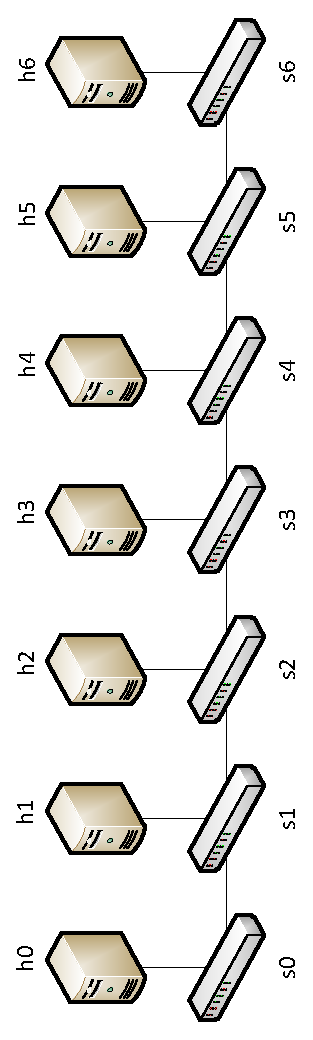
\includegraphics[angle=-90, width=0.45\textwidth, clip]{figs/line.eps}
}

%\subfloat[][Ring Topology] {
%	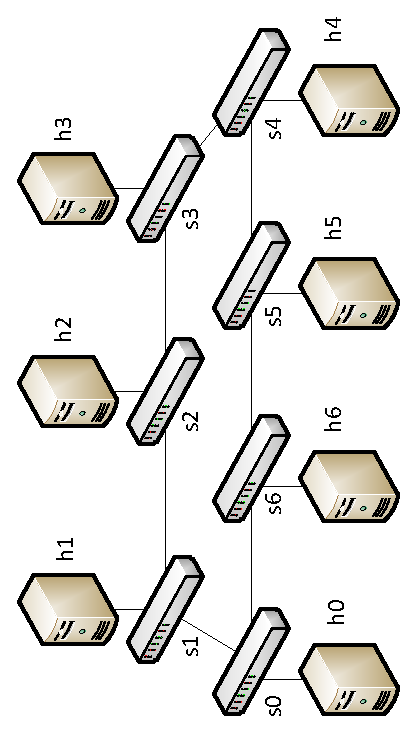
\includegraphics[angle=-90, width=0.30\textwidth, clip]{figs/ring.eps}
%}

\subfloat[][Tree Topology] {
	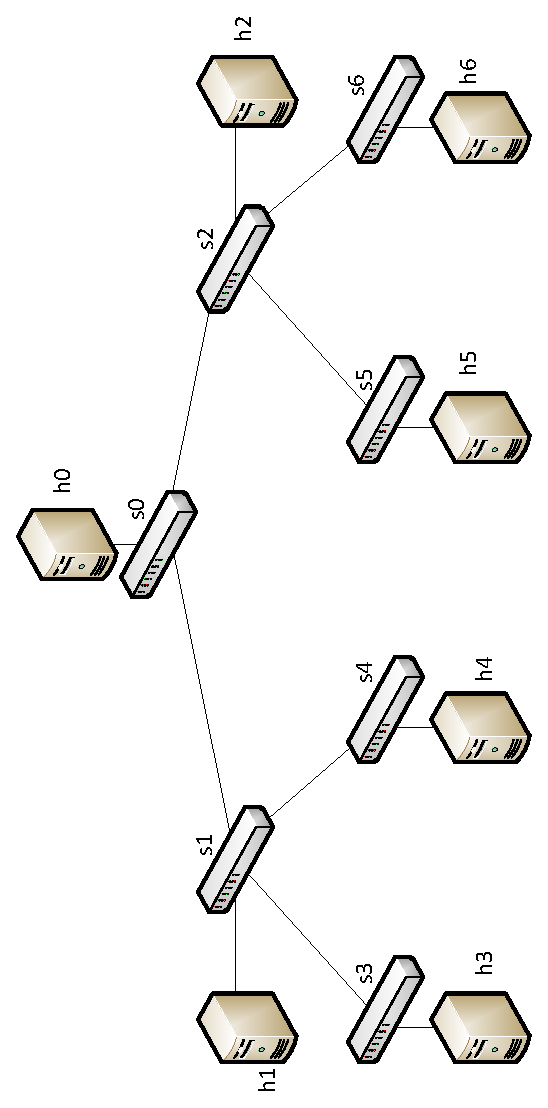
\includegraphics[angle=-90, width=0.48\textwidth, clip]{figs/tree.eps}
}

\subfloat[][Star Topology] {
	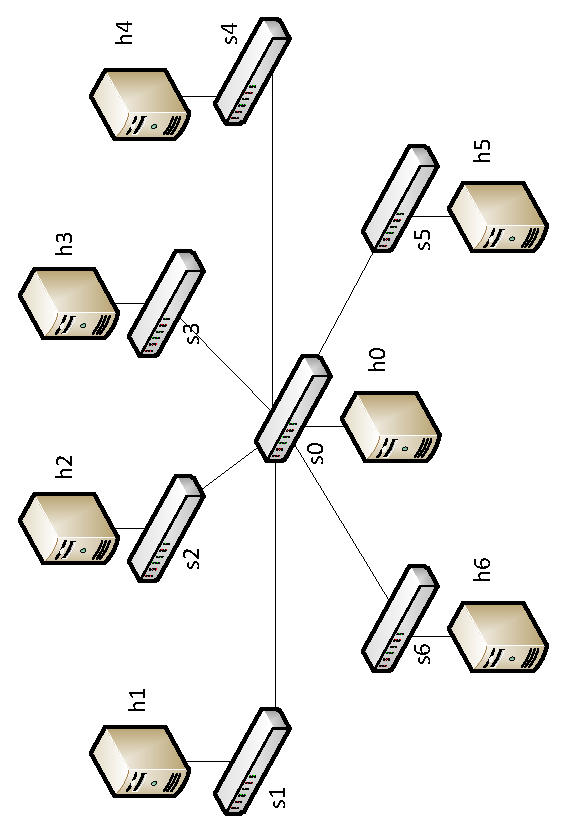
\includegraphics[angle=-90, width=0.35\textwidth, clip]{figs/star.eps}
}

\caption{Different Network Topologies Considered in This Report} 
\label{fig:topo}
\end{figure}
